\documentclass[a4paper]{article}
\title{\Huge{\textsc{Evolutionary Algorithms for Iterated Prisoner's Dilemma}}}
\usepackage[margin=3cm]{geometry}
\usepackage{graphicx}
\usepackage{wrapfig}
\usepackage{caption}
\usepackage{amsmath}
\usepackage{subcaption}
\usepackage[export]{adjustbox}
\usepackage{enumerate}
\usepackage{url}
\usepackage{authblk}
\usepackage{float}
\usepackage{wrapfig}
\usepackage{setspace}
\usepackage{mdframed}
\usepackage{booktabs}
\usepackage{ragged2e}

\graphicspath{{learnerPlots/}}

\def\changemargin#1#2{\list{}{\rightmargin#2\leftmargin#1}\item[]}
\let\endchangemargin=\endlist 

\DeclareMathSizes{10}{10}{10}{10}
\begin{document}

    \newgeometry{left=4cm,right=4cm,top=4cm,bottom=5cm}
	\begin{titlepage}
	    \begin{center}
	        \vspace*{5mm}
	        
	        \vspace{5mm}
	        {\huge{\textsc{Evolutionary Algorithms}}}\\
	        \vspace{2mm}
	        {\Large{\textsc{for Infinitely Repeated Prisoner's Dilemma}}}\\
	        \vspace{8mm}
	        {\large{Nishant Rai}}\\
			\vspace{3mm}
			
			{\normalsize{Department of Computer Science and engineering\\}}
	        \vspace{4mm}
        	\vspace{7mm}
	        \textbf{Abstract\\}
        	\vspace{4mm}
        	\noindent
{\justifying{The project deals with the problem of computing successful strategies for Iterated Prisoner's dilemma. We start off by discussing existing work in the area along with some results and popular methods used for computing efficient strategies. We simulate multiple results and also confirm previous findings and claims. The discussed algorithms include Evolutionary Strategies and Reinforcement Learning (Which compute optimal and also adaptive strategies which perform well against multiple opponents). We propose new algorithms based on Reinforcement Learning to compute good strategies which perform well against a set of baseline algorithms (Including the extremely simple yet effective 'Tit for Tat'). This strategy is also compared against Axelrod's Evolutionary Strategy. We discuss Axelrod's Tournament and use a similar setup to decide the effectiveness of the computed strategies. The result section shows the superiority of the strategies computed using them. We also discuss the shortcomings and strengths of the algorithms.} \par}
			\vfill
			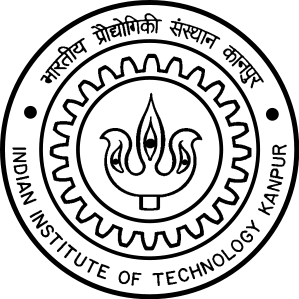
\includegraphics[width=0.25\textwidth]{iitklogo.png}\\[0.1in]
            \vspace{3mm}
	        {\Large{\textsc{ECO502A: Case Study}}\\}
			\vspace{3mm}            
            \normalsize{Under the guidance of Dr. Vimal Kumar\\}
            \vspace{1mm}
            {Indian Institute of Technology, Kanpur}
	    \end{center}
	\end{titlepage}
	\restoregeometry

	\tableofcontents
	
	\pagebreak	
	
	\section{Introduction}
	
	The Prisoner's Dilemma is a classic problem in game theory, which is mainly a paradox demonstrating that two individuals acting in their own interest might choose an action which is worse off than any other. It has become a popular problem because there has been showing its similarity to real-world problems. The standard game is set up such that both players choose to protect themselves (Instead of cooperating) at the expense of their partner. Even though the thought process involved seems to be extremely logical, but both players eventually find themselves in a worse state than if they had cooperated with each other.\\
	
	We consider the following instance of Prisoner's Dilemma (Note that the essence remains the same). Players A and B have been arrested in connection with a crime. Both of them are put in a separate interview room and told that a deal may be available to them depending on whether each provides testimony against the other (Defects) or keeps silent (Cooperates). We assume that each  individual wants do as well as possible for only themselves (i.e. without any regard for the welfare of the other player). For further discussions, we denote the possible actions as $C_{x}$ and $D_{x}$ i.e. Player $x$ cooperating or defecting. The payoffs for the game are given in Table 1 below,

	\tabcolsep=0.51cm
	\begin{table}[H]
	\centering
	\begin{tabular}{|c|c|c|}
	\hline
					& $C_{B}$           		& $D_{B}$ 					\\ \hline
	$C_{A}$  		& (3,3) 		 			& (0,5)         			\\ \hline
	$D_{A}$			& (5,0)           			& (1,1)            			\\ \hline
	\end{tabular}
	\caption{Payoff matrix for the Prisoner's Dilemma}
	\end{table}
		
	For ease of discussion afterwards, we define the following terms based on the actions chosen by the players (They are described in Table 2),
	\begin{itemize}
		\item T : \textbf{Temptation} for unilateral defection
		\item R: \textbf{Reward} for mutual cooperation
		\item P : \textbf{Punishment} for mutual defection
		\item S: \textbf{Sacrifice} for unilateral cooperation	
	\end{itemize}
	
	\begin{table}[H]
	\centering
	\begin{tabular}{|c|c|c|}
	\hline
					& $C_{B}$           		& $D_{B}$ 					\\ \hline
	$C_{A}$  		& (R,R) 		 			& (S,T)         			\\ \hline
	$D_{A}$ 		& (T,S)           			& (P,P)            			\\ \hline
	\end{tabular}
	\caption{State definitions for the Prisoner's Dilemma}
	\end{table}

	As discussed earlier, we can conclude that the moves chosen by the players would be $(D_{A},D_{B})$. This can be termed as the Nash Equilibrium of the game. An interesting variant of the classical prisoner's game arises when the game is repeated multiple times. It is termed as Iterated Prisoner's Dilemma. The situation becomes even more interesting when the game satisfies the following conditions,
	\begin{enumerate}
	\item The winner is the player with the highest score in the end.
	\item The number of moves should 'not' be known to the two players.
	\item Usually, there are many players in the fray, and there is a Round Robin Tournament among all the players - the player with the highest score wins.		
	\end{enumerate}
	
	Due to the fact that the players do not know the number of repetitions of the game, thus it becomes equivalent to playing the game infinite times.	This is the game we will be studying in this Case study: The Infinitely Repeated Prisoner's Dilemma.
	
	\section{Existing Work}
	
	There has been a huge amount of work on It can be argued that Axelrod has been the most influential researcher in the area of the Iterated Prisoner's Dilemma. In Axelrod's original work, two tournaments based on IPD were undertaken; which later defined the methods by which IPD strategies ought to be compared. In this process, Axelrod invited professional game theorists to submit programs for playing a computer-based Iterated Prisoner's Dilemma. Axelrod's work has also been extremely influential in other studies.\\
	Later, Axelrod used a Genetic Algorithm (GA), an artificial intelligence technique (Inspired by biological evolution), to simulate agent learning. The algorithm uses operators such as mutation and crossover (Derived from evolution). In investigating evolutionary future round tournaments, Axelrod considered a set of strategies that is deterministic and uses outcomes of the past 'three' moves (Discussed later) to determine a current move.\\
	Further works adapt the same approach. This means that all strategies encoded in these environments are history dependent. In other word, such environment consists only of memory-based strategies. However, alternative representation of strategies could exist. Kraines showed that ‘Pavlovian’ strategies are able to support the evolution of cooperation in tournaments where players are making errors. 
	
	\section{Axelrod's Tournament}

	In 1980, Robert Axelrod, professor of political science at the University of Michigan, held a tournament of various strategies for the prisoner's dilemma. He invited a number of well-known game theorists to submit strategies to be run by computers. In the tournament, programs played games against each other and themselves repeatedly. Each strategy specified whether to cooperate or defect based on the previous moves of both the strategy and its opponent.\\
	Some of the strategies submitted were:
	\begin{itemize}
	\item \textbf{Always Defect}: This strategy defects on every turn. This is what game theory advocates. It is the safest strategy since it cannot be taken advantage of. However, it misses the chance to gain larger payoffs by cooperating with an opponent who is ready to cooperate.
	\item \textbf{Always Cooperate:} This strategy does very well when matched against itself. However, if the opponent chooses to defect, then this strategy will do badly.
	\item \textbf{Random:} The strategy selects its move randomly i.e. cooperates and defects 50\% of the time.
	\end{itemize}
	
	All of these strategies are prescribed in advance. Therefore, they cannot take advantage of knowing the opponent's previous moves and figuring out its strategy. The winner of Axelrod's tournament was the 'Tit for Tat' strategy. The strategy cooperates on the first move, and then does whatever its opponent has done on the previous move. Thus, when matched against the all-defect strategy, 'Tit for Tat' strategy always defects after the first move. When matched against the all-cooperate strategy, 'Tit for Tat' always cooperates. This strategy has the benefit of both cooperating with a friendly opponent, getting the full benefits of cooperation, and of defecting when matched against an opponent who defects. When matched against itself, the 'Tit for Tat' strategy always cooperates.\\
	'Tit for Tat' relies on the assumption that its opponent is trying to maximize his score. When paired with a mindless strategy like 'Random', 'Tit for Tat' sinks to its opponent's level. For that reason, 'Tit for Tat' cannot be called a 'best' strategy. It must be realized that there really is no 'best' strategy for prisoner's dilemma. Each individual strategy will work best when matched against a 'worse' strategy. In order to win, a player must figure out his opponent's strategy and then pick a strategy that is best suited for the situation.
	
	\subsection{Features of Successful Strategies}

A strategy (pure) for a player in a particular game is a plan describing what move that player should take in each possible situation (information state) that might arise for him.
In Axelrod’s IPD tournaments, strategies exhibiting the following four properties tended to be more successful (i.e., to accumulate higher total payoffs), with the clear-cut winner being the Tit-for-Tat strategy.
	\begin{itemize}
		\item \textbf{Niceness}: Never be the first to defect.
		\item \textbf{Provocability}: Get mad quickly at defectors and retaliate.
		\item \textbf{Forgiveness}: Do not hold a grudge once you have vented your anger.
		\item \textbf{Clarity}: Act in ways that are straightforward for others to understand.
	\end{itemize}

	\subsection{Axelrod Strategies}	

As we have seen earlier that 'Tit for Tat', such a simple strategy turned out to be the winner in Axelrod's tournament. Axelrod set out to find other simple strategies with similar or greater power.\\
Axelrod adopted a simple but elegant way for encoding strategies, and then used a single-objective evolutionary algorithm to obtain optimal strategies. His encoding scheme remained a standard way of handling the IPD problem and is described below. We also adopt a similar encoding scheme to compute optimal strategies for the game. Axelrod's method had the following features,
	\begin{itemize}
	\item The next move depends upon the behavior of both the parties during previous three (In general k, termed as memory length in this paper) moves.
	\item We have four possibilities for the previous move, which are as follows,
	\begin{itemize}
		\item CC or R for Reward
		\item CD or S for Sucker
		\item DC or T for Temptation
		\item DD or P for Penalty
	\end{itemize}		
	\item We code the particular behavioral sequence as a 3-letter string.	
	\item We then use the 3-letter sequence to generated a number between 0 and 63 (i.e. $4^{3} = 4^{k}$) by interpreting it as an integer base 4 (Since there were 4 possibilities for each turn).
	\item Strategy string : 64-bit binary string of C's and D's where he $i^{th}$ bit corresponds to the $i^{th}$ behavioral sequence.
	\end{itemize}

	The following \textbf{critical} points should be observed,
	\begin{itemize}
	\item The behavior of the player is undefined in the first three moves of the game (Since we do not have histories of the game).
	\item We also add six bits to the encoding to specify a strategy's premises, i.e. assumption about the pre-game behavior.
	\item Together, each of the 70-bit strings represent a particular strategy (i.e. State-action codes)	
	\end{itemize}		
	
	\section{Motivation}
	
	As discussed in the previous section, Axelrod's encoding can be used to define a strategy. We decide to use Evolutionary Algorithms to compute the optimal (Axelrod) strategy because the total number of all possible strategies very high (i.e. $2^{70}$). If we perform exhaustive search, it will take a huge amount of time (A couple billion years or more!). We do not seek help from standard optimization procedure since the fitness function required is not continuous or differentiable, thus classical methods will not work. Hence, genetic (evolutionary) algorithms are a good choice.
	
	\section{Proposed Algorithms}
	
	\subsection{Axelrod Strategies using Evolutionary Algorithms}

	As mentioned earlier, Axelrod's approach involved maximizing the self score using a Single Objective Genetic Algorithm. We study Axelrod's model along with optimizing multiple objectives (i.e. Self Score and Opponent score) simultaneously using NSGA-II algorithm. We later compare the computed strategies.\\
	The intuition for using another objective (i.e. Opponent score) is that the Prisoner's dilemma game is similar to a constant sum game (If we exclude the case when both confess), thus minimizing the opponent score might indirectly help us in maximizing our own score.

	\subsection{Reinforcement Learning for Adaptive Strategies}
	
	\section{Experiments}
	
	Both Single Objective Evolutionary Algorithm and Multi Objective Evolutionary Algorithm (MEA) are used for getting optimal strategies. The proposed strategies are evaluated in the later sections as discussed below.\\
	We describe the rough structure of the evolutionary algorithms. In each generation, a certain number (referred to as population size) of strategies are generated, and each strategy was made to play against \textbf{n} other players. Each game consisted of \textbf{p} moves. Then the next generation is created using a recombination operator involving the best strategies from the earlier one. The payoff matrix is the same as shown in Table 1. The details of the \textbf{n} other players have been given in the section: \textit{Baseline Strategies}.

	\subsection{Baseline Strategies}
	
	The baseline strategies used in the experiments are as follows,
	\begin{enumerate}
	
	\item \textbf{Always Cooperate:} Cooperates on every move
	\item \textbf{Always Defect:} Defects on every move
	\item \textbf{Tit for Tat:} Cooperates on the first move, then simply copies the opponent's last move.
	\item \textbf{Suspicious Tit for Tat:} Same as Tit for Tat, except that it defects on the first move
	\item \textbf{Random:} Makes a random move.
	\item \textbf{Cyclic CCD:} Plays C, C, D periodically.
	\item \textbf{Tit for Two Tats:} Cooperates on the first move, and defects only when the opponent defects two times.
	\item \textbf{Soft Majority:} Begins by cooperating, and cooperates as long as the number of times the opponent has
cooperated is greater than or equal to the number of times it has defected, else it defects.
	\item \textbf{Hard Majority:} Defects on the first move, and defects if the number of defections of the opponent is greater than or equal to the number of times it has cooperated, else cooperates.
	\item \textbf{Hard Tit for Tat:} Cooperates on the first move, and defects if the opponent has defects on any of the previous three moves, else cooperates.
	\item \textbf{Prober:} Plays D, C, C initially. Defects forever if opponent cooperated in moves 2 and 3. Otherwise plays Tit for Tat.	
	\end{enumerate}
	
	\subsection{Tournament Setup}
	
	The tournament setup is inspired by Axelrod's initial study. It consists of a round robin tournament amongst all the strategies where each game is played for 200 turns. The whole tournament is repeated a few times (10 times in our experiments) to lessen the effect of randomness.

	\section{Results for Evolutionary Algorithm}

	\subsection{Evolution Statistics}

	\subsubsection{Single Objective Genetic Algorithm}	

	\begin{wrapfigure}{R}{0.55\textwidth}
	\centering
	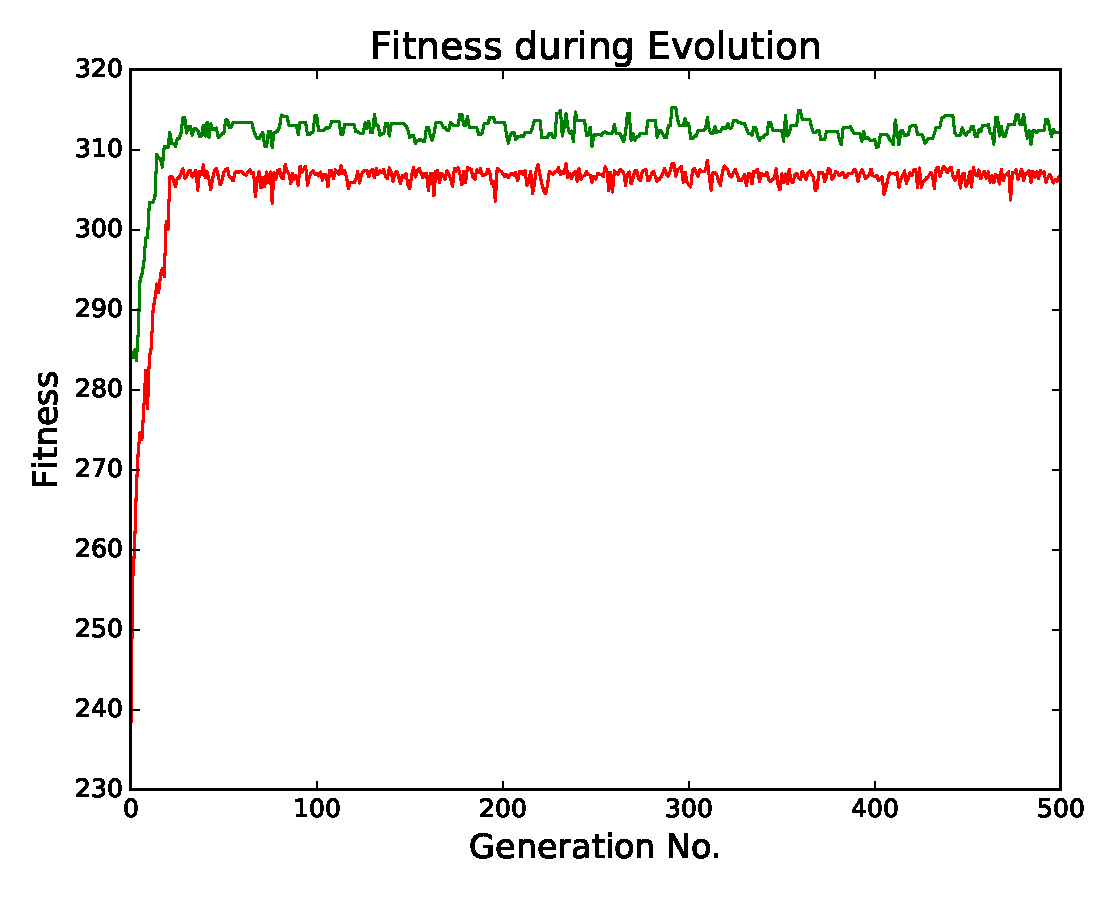
\includegraphics[width=0.53\textwidth]{singFitPlot.eps}
	\caption{\footnotesize{Fitness of Population during Evolution}}
	\end{wrapfigure}
	The single-objective Evolutionary Algorithm used is the same as used by Axelrod in his initial study. As done earlier, the fitness i.e. self-score of the player is maximized during evolution. For the experiment, the population size was fixed at 60. The results obtained when the evolutionary algorithm is run for 500 generations is shown in figure.\\
	We show the maximum and average fitness of the population. As we can see the population achieves the final value extremely quickly (Under 50 iterations). The fluctuations caused in between are a result of the mutations introduced in the population (Something inherent in Evolutionary Algorithms).\\
	After 500 generations the maximum fitness amongst all the samples in the population is around 312, which is even higher than the benchmark score (300) \textbf{(Dawkins)}. This shows the superiority of the Evolutionary strategy and is also in line with the results obtained by Axelrod. When this strategy is pitted against other strategy in an Axelrod-like tournament, the evolved strategy emerges as a clear winner (By a huge margin). The results are discussed in later sections.	

	\subsubsection{Multi Objective Genetic Algorithm}
		
	\begin{wrapfigure}{R}{0.55\textwidth}
	\centering
	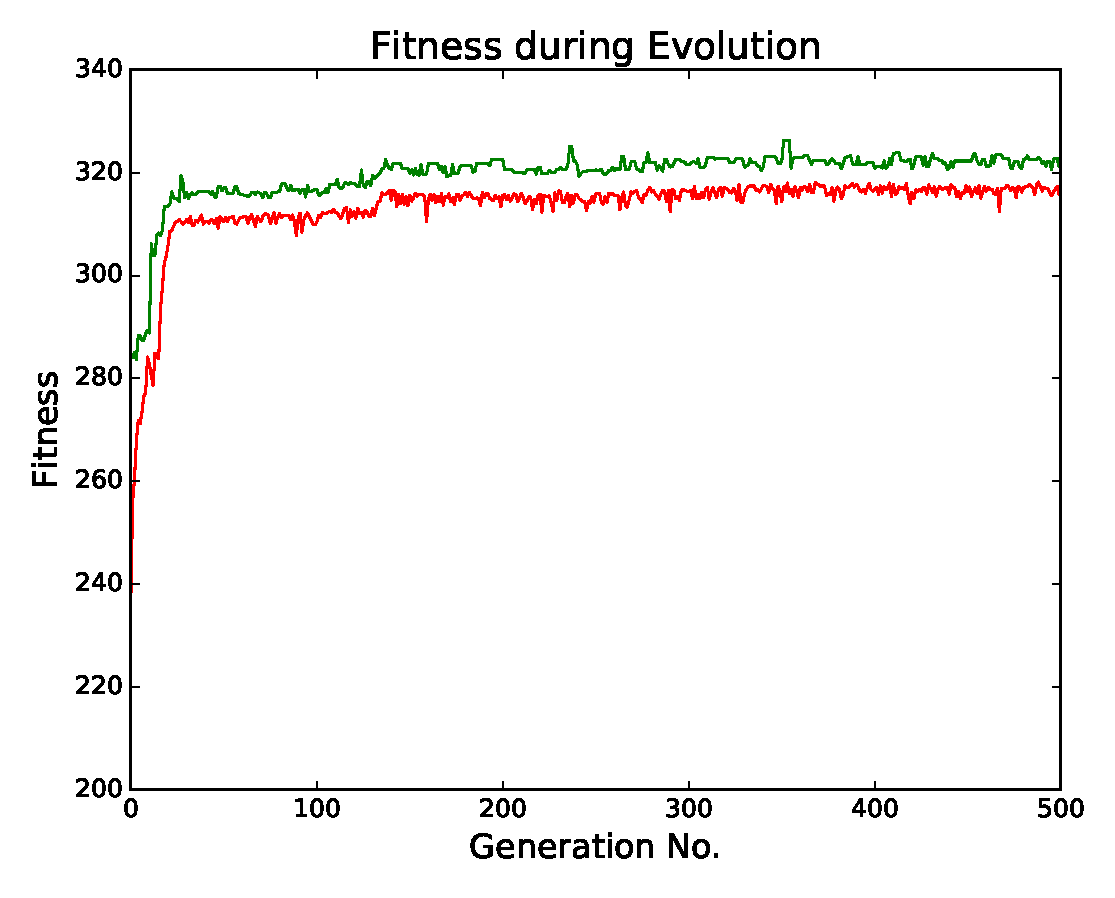
\includegraphics[width=0.53\textwidth]{multFitPlot.eps}
	\caption{\footnotesize{Fitness of Population during Evolution}}
	\end{wrapfigure}
	Instead of just maximizing our own score as proposed by Axelrod, we perform another experiment in which along with maximizing our self score we also try to reduce the opponents score. The intuition for this can be seen from the payoff matrix of the game. Assume that the opponent has selected his move and it's our turn to choose. Notice that for all moves of the opponent, the one in which we get higher payoff is the one in which our rival gets a lower payoff.\\
	We used a Multi-Objective Evolutionary Algorithm (NSGA-II) to compute the strategy. For the experiment, the population size was fixed at 60. The results obtained when the evolutionary algorithm is run for 500 generations is shown in figure. We show the maximum and average fitness of the population. The behavior of evolution mostly remains similar to the previous case. But we can see that the final value obtained \textit{(321)} in this case is higher than the Single Objective counterpart \textit{(312)}, which further motivates the benefit of using a multi-objective optimization algorithm.\\

	To further demonstrate the evolution, we plot the initial and final strategies obtained in Figure 3. The blue crosses represent the initial randomly initialized strategies. The red pluses represent the final evolved strategies, it can be easily seen that the initially random population slowly approaches the 'optimal' region. The out of place red members in the final evolved population are the mutated individuals.

	\begin{figure}[H]
	\centering
	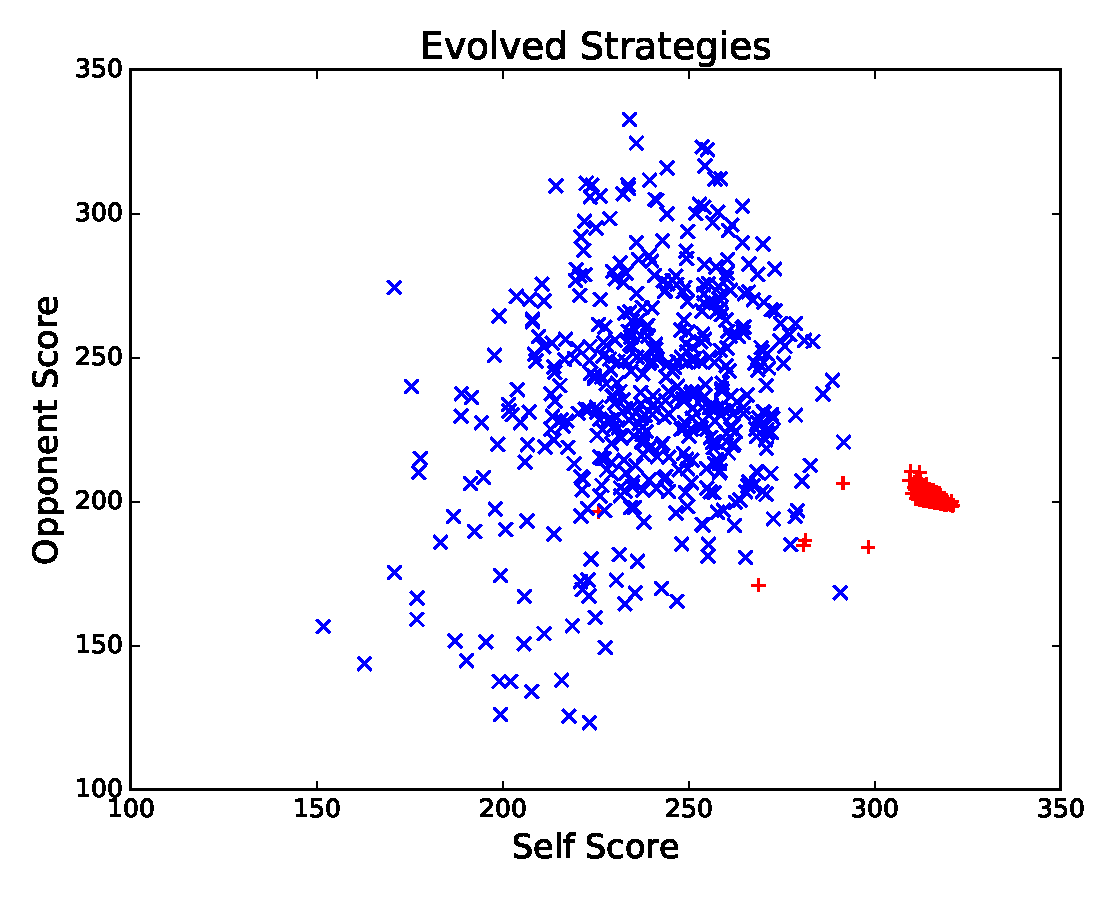
\includegraphics[width=0.75\textwidth]{evolvePlot.eps}
	\caption{{Distribution of Final Evolved Strategies and the Initial Randomly initialized Strategies}}
	\end{figure}

	\subsection{Effect of Memory on Strategies}
	
	Axelrod performed his experiments assuming a memory length of 3. We perform our experiments with multiple memory lengths to gain insight whether it is in fact optimal. The results are shown in the following table,
	
	\begin{table}[H]
	  \begin{center}
	    \begin{tabular}{c|c|c}
	      \toprule
	      \textsc{Memory Length} & \textsc{Self Score} & \textsc{Encoding Size}\\
	      \midrule
	      1 & 280.18 & 6\\
		  2 & 291.36 & 20\\
		  \textbf{3} & \textbf{314.27} & \textbf{70}\\
		  4 & 281.72 & 264\\
		  5 & 284.09 & 1034\\
		  6 & 296.18 & 4108\\		  
		  \bottomrule
	    \end{tabular}
	    \caption{\textsc{Effect of Memory}}
	  \end{center}
	\end{table}  
	
	\subsection{Tournament amongst strategies}

	We conduct an Axelrod-like tournament amongst the mentioned strategies to compare and evaluate them. The baseline strategies used are mentioned in the earlier sections.

	\subsubsection{Multi Objective Strategy Vs Others}

	In this setup we conduct a tournament between the strategy computed using the Multi Objective GA and the baseline strategies. The best performer has been highlighted in bold text. The average score refers to the average payoff per turn.

	\begin{table}[H]
	  \begin{center}
	    \begin{tabular}{c|c}
	      \toprule
	      \textsc{Player} & \textsc{Average Score}\\
	      \midrule
			Cooperator & 2.091\\
			Defector & 1.799\\
			Cycler CCD & 2.339\\
			Hard Go By Majority & 2.023\\
			\textbf{Multi Objective Strategy} & \textbf{3.183}\\
			Soft Go By Majority & 2.418\\
			Hard Tit For Tat & 2.317\\
			Tit For 2 Tats & 2.304\\
			Suspicious Tit For Tat & 2.269\\
			Random: 0.5 & 2.244\\
			Tit For Tat & 2.627\\
			Prober & 2.510\\
		  \bottomrule
	    \end{tabular}
	    \caption{\textsc{Tournament Results}}
	  \end{center}
	\end{table}  

	\subsubsection{Single Objective Strategy Vs Others}

In this setup we conduct a tournament between the strategy computed using the Single Objective GA and the baseline strategies. The best performer has been highlighted in bold text. The average score refers to the average payoff per turn.
	
	\begin{table}[H]
	  \begin{center}
	    \begin{tabular}{c|c}
	      \toprule
	      \textsc{Player} & \textsc{Average Score}\\
	      \midrule
			Cooperator & 2.089\\
			Defector & 1.807\\
			Cycler CCD & 2.333\\
			Hard Go By Majority & 2.037\\
			\textbf{Single Objective Strategy} & \textbf{3.159}\\
			Soft Go By Majority & 2.426\\
			Hard Tit For Tat & 2.319\\
			Tit For 2 Tats & 2.304\\
			Suspicious Tit For Tat & 2.273\\
			Random: 0.5 & 2.273\\
			Tit For Tat & 2.630\\
			Prober & 2.500\\
		  \bottomrule
	    \end{tabular}
	    \caption{\textsc{Tournament Results}}
	  \end{center}
	\end{table}  

	\subsubsection{Tournament with all strategies}
	
In this setup we conduct a tournament consisting of both the evolutionary strategy and the baseline strategies. The best performer has been highlighted in bold text. The average score refers to the average payoff per turn.	
	
	\begin{table}[H]
	  \begin{center}
	    \begin{tabular}{c|c}
	      \toprule
	      \textsc{Player} & \textsc{Average Score}\\
	      \midrule
			Cooperator & 2.043\\
			Defector & 1.737\\
			Cycler CCD & 2.179\\
			Hard Go By Majority & 1.977\\
			\textbf{Multi Objective Strategy} & \textbf{3.051}\\
			Soft Go By Majority & 2.356\\
			Hard Tit For Tat & 2.375\\
			Tit For 2 Tats & 2.235\\
			{Single Objective Strategy} & {3.045}\\
			Suspicious Tit For Tat & 2.331\\
			Random: 0.5 & 2.201\\
			Tit For Tat & 2.661\\
			Prober & 2.551\\
		  \bottomrule
	    \end{tabular}
	    \caption{\textsc{Tournament Results}}
	  \end{center}
	\end{table}  

	It can be seen that the Multi Objective Strategy performs slightly better than the Single counterpart. This reaffirms the superiority of the Multi Objective strategy over the Single Objective one.
	
	\subsection{Observations}
	
	\subsubsection{Behavior of the Evolved strategies}

	We choose a few individuals out of the evolved population randomly and compare the strategies obtained. We mention some of the interesting traits found common in all the strategies. We also try to relate the trends observed in these strategies to the desirable qualities required for successful strategies (Mentioned in previous sections). Some of the trends noted in the strategies are as follows,
	\begin{itemize}
	\item \textbf{PPP (0) :} In this situation both the players have been defecting over the previous three moves. Since both players were defecting previously, defecting again would be a good choice to minimize the damage and prevent the opponent's score to increase.
	\item \textbf{PPT (1) :} In this case, the opponent defected on the first two moves, but cooperated in the third move, while player 1 defected in all the three moves. Thus, we should continue to exploit the 'foolishness' of the opponent and defect in the next move too (Expecting the opponent to cooperate).
	\item \textbf{PTP, PTT (4, 5) :} Here, all of the given cases are similar to the previous case, which means defecting would be the best choice (To exploit the 'foolish' opponent).
	\item \textbf{PRR (15) :} Here, the opponent has cooperated for the last few moves, so in order to gain more points defecting will be a good choice. But, note that this may make the opponent distrustful.
	\item \textbf{TPT, TTT (17, 21) :} All the given cases are similar to the previous case, which means defecting would be the best choice (To exploit the 'foolish' opponent).
	\item \textbf{TTP (20) :} Here, the opponent was cooperating with us initially. But it didn't in the last move, which shows that trust has been lost and the best move would be to defect again.
	\item \textbf{TRR (31) :} After being betrayed, we and the opponent both start cooperating. Thus, to exploit this relationship it would be best to defect next.
	\item \textbf{STT (37) :} This case is quite similar to the 'foolish' opponent cases discussed above. So, the best choice is to defect.
	\item \textbf{SRR (47) :} After being betrayed, we and the opponent both start cooperating. Thus, we should continue cooperating. Note the difference between 31 and 47. Even though the last two turns (histories) are the same, the next action is completely different. It can be speculated that this is due to the fact that in 31, the opponent trusts us easily (Since it cooperated after being betrayed). So, we can betray it again, hoping that it won't mind. But in this case, we are not aware of the opponent's behavior (Since we were betrayed here).
	\item \textbf{RTR (55) :} This case is again similar to the 'foolish' opponent case. In this case, the opponent trusts us easily. So, exploiting this behavior would be the best.
	\item \textbf{RRT (61) :} Here, both players have cooperated in the initial two moves and we've exploited it in the last turn. So, now that trust has been lost it would be better to defect.
	\item \textbf{RRR (63) :} In this case, both players have cooperated in the last few moves. So, the best move would be to continue cooperating (So that we don't lose trust).
	\end{itemize}
	
	\subsubsection{Effect of Memory on Strategies}	

	As we can see in the table shown earlier. As we increase the memory length, an interesting trend is observed. At first, the memory increases till an optimum value (i.e. 3) then it suddenly decreases. Then, after the sudden decrease it gradually increases once again.\\
	Notice that ideally, higher memory must result in better performance. Because it's trivial to show that the set of strategies using memory $n$ must be a subset of the set of strategies using memory $n+1$. But unfortunately this is the opposite of what is observed in the experiments. We suspect that the reason for poor performance despite the earlier mentioned fact is the limitations of the Genetic Algorithm.\\
	As memory length increases, the corresponding solution space also increases exponentially. This results in the algorithm being prone to get stuck in local minimas. It also means that the Genetic Algorithm would require more generations (iterations) to arrive at a reasonable solution. Thus, the value proposed by Axelrod (i.e. 3) seems to be the optimal memory length considering the trade-off between Computational Power and Performance.
	
	\section{Results for Adaptive Strategies}

	\subsection{Learning Performance}
		
	\subsubsection{Performance Against Other Strategies}
	
	In our experiments we conduct matches of our adaptive strategies against other strategies (Shown in the figure). We try different variants of the adaptive strategy and evaluate them. The plots shown below show the average score over a fixed interval (1000-5000) to reduce the variance. 
	
	\begin{figure}[H]
	\centering
	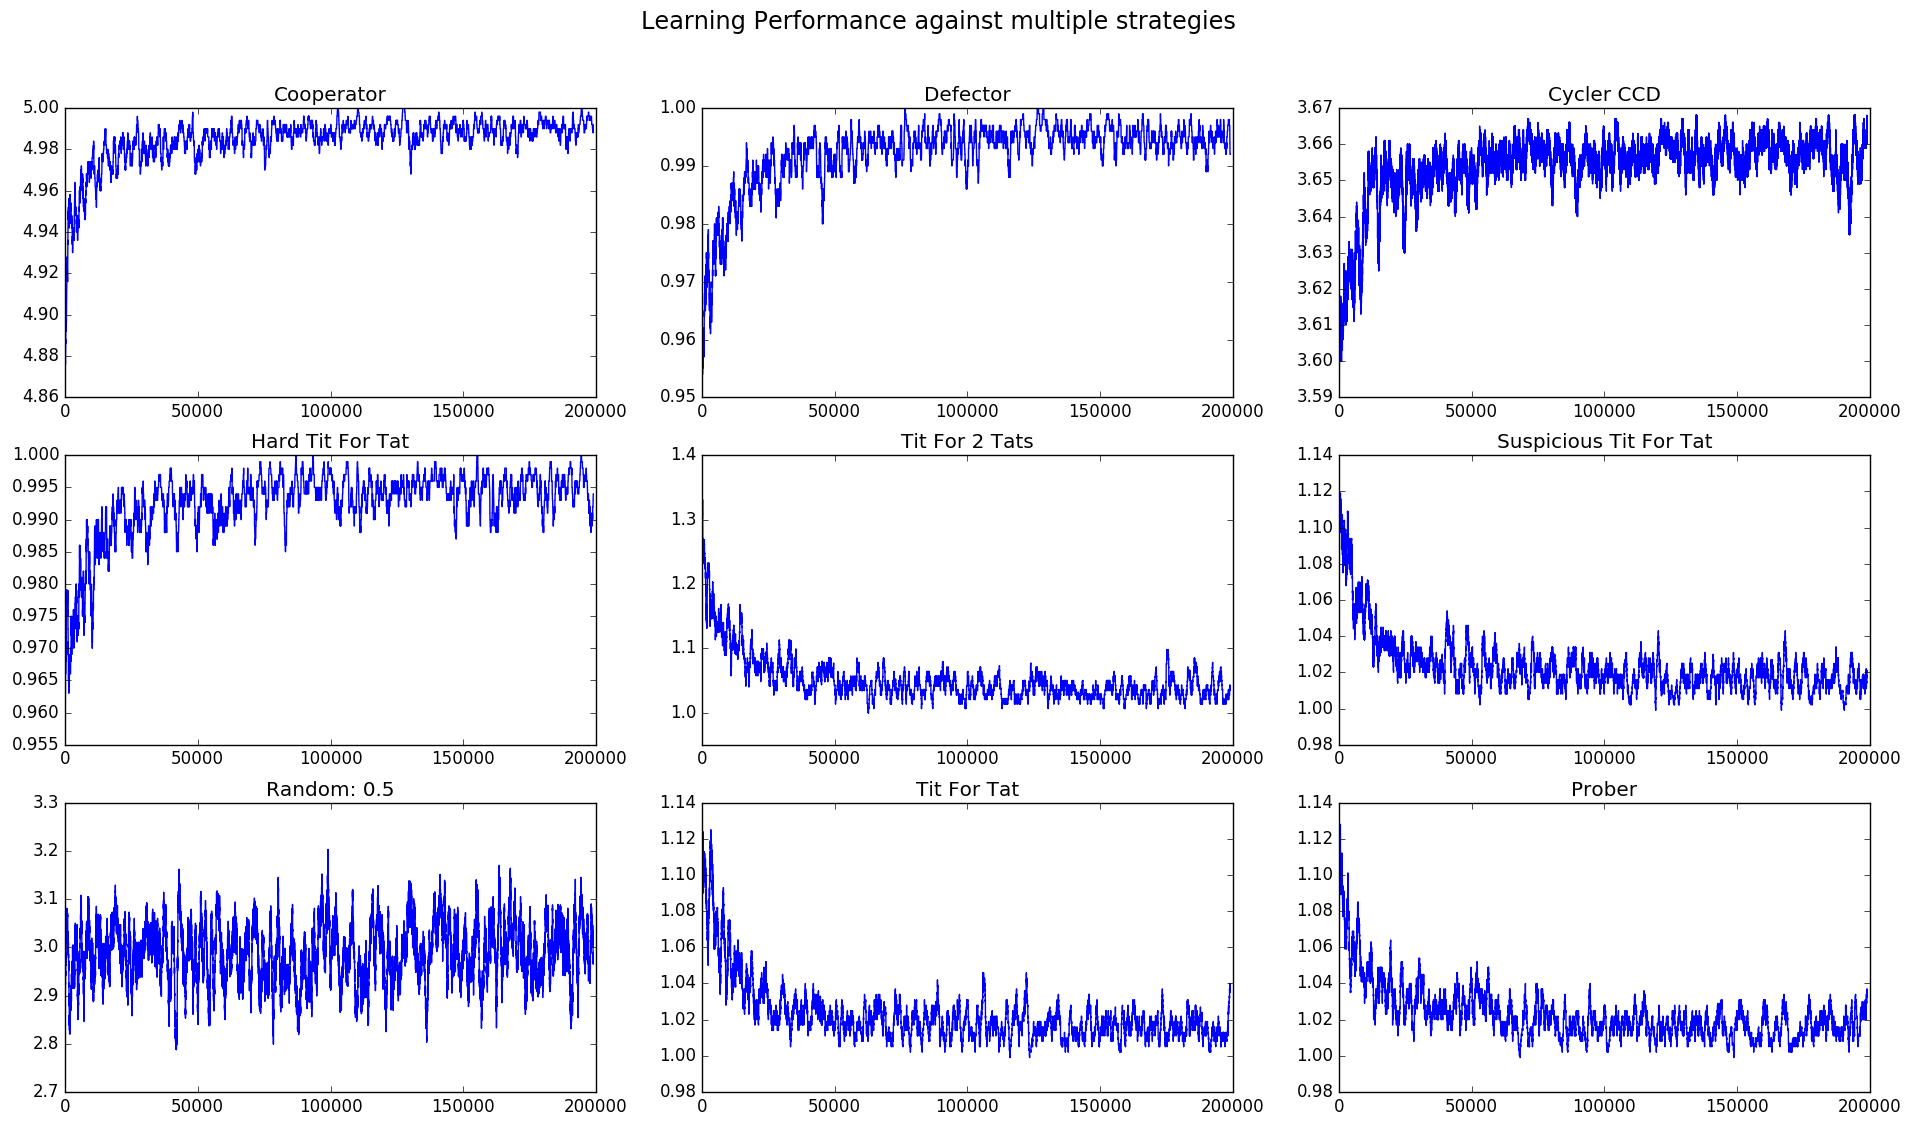
\includegraphics[width=\textwidth]{learnerB.png}
	\caption{{Performance of Adaptive strategy (Variant B)}}
	\end{figure}

	\subsubsection{Initial Behavior (Payoff)}

	As discussed earlier, the proposed adaptive strategy learns the optimal way to play based on an Explore-Exploit agenda. Thus, it is critical to observe how quickly it adapts/learns to play. The following plots show the initial behavior of our adaptive strategy against multiple opponents. A gradual increase in the score is desirable. We do not show results for Variant A due to its random nature, which make the corresponding plots slightly messy.\\

	\begin{figure}[H]
	\centering
	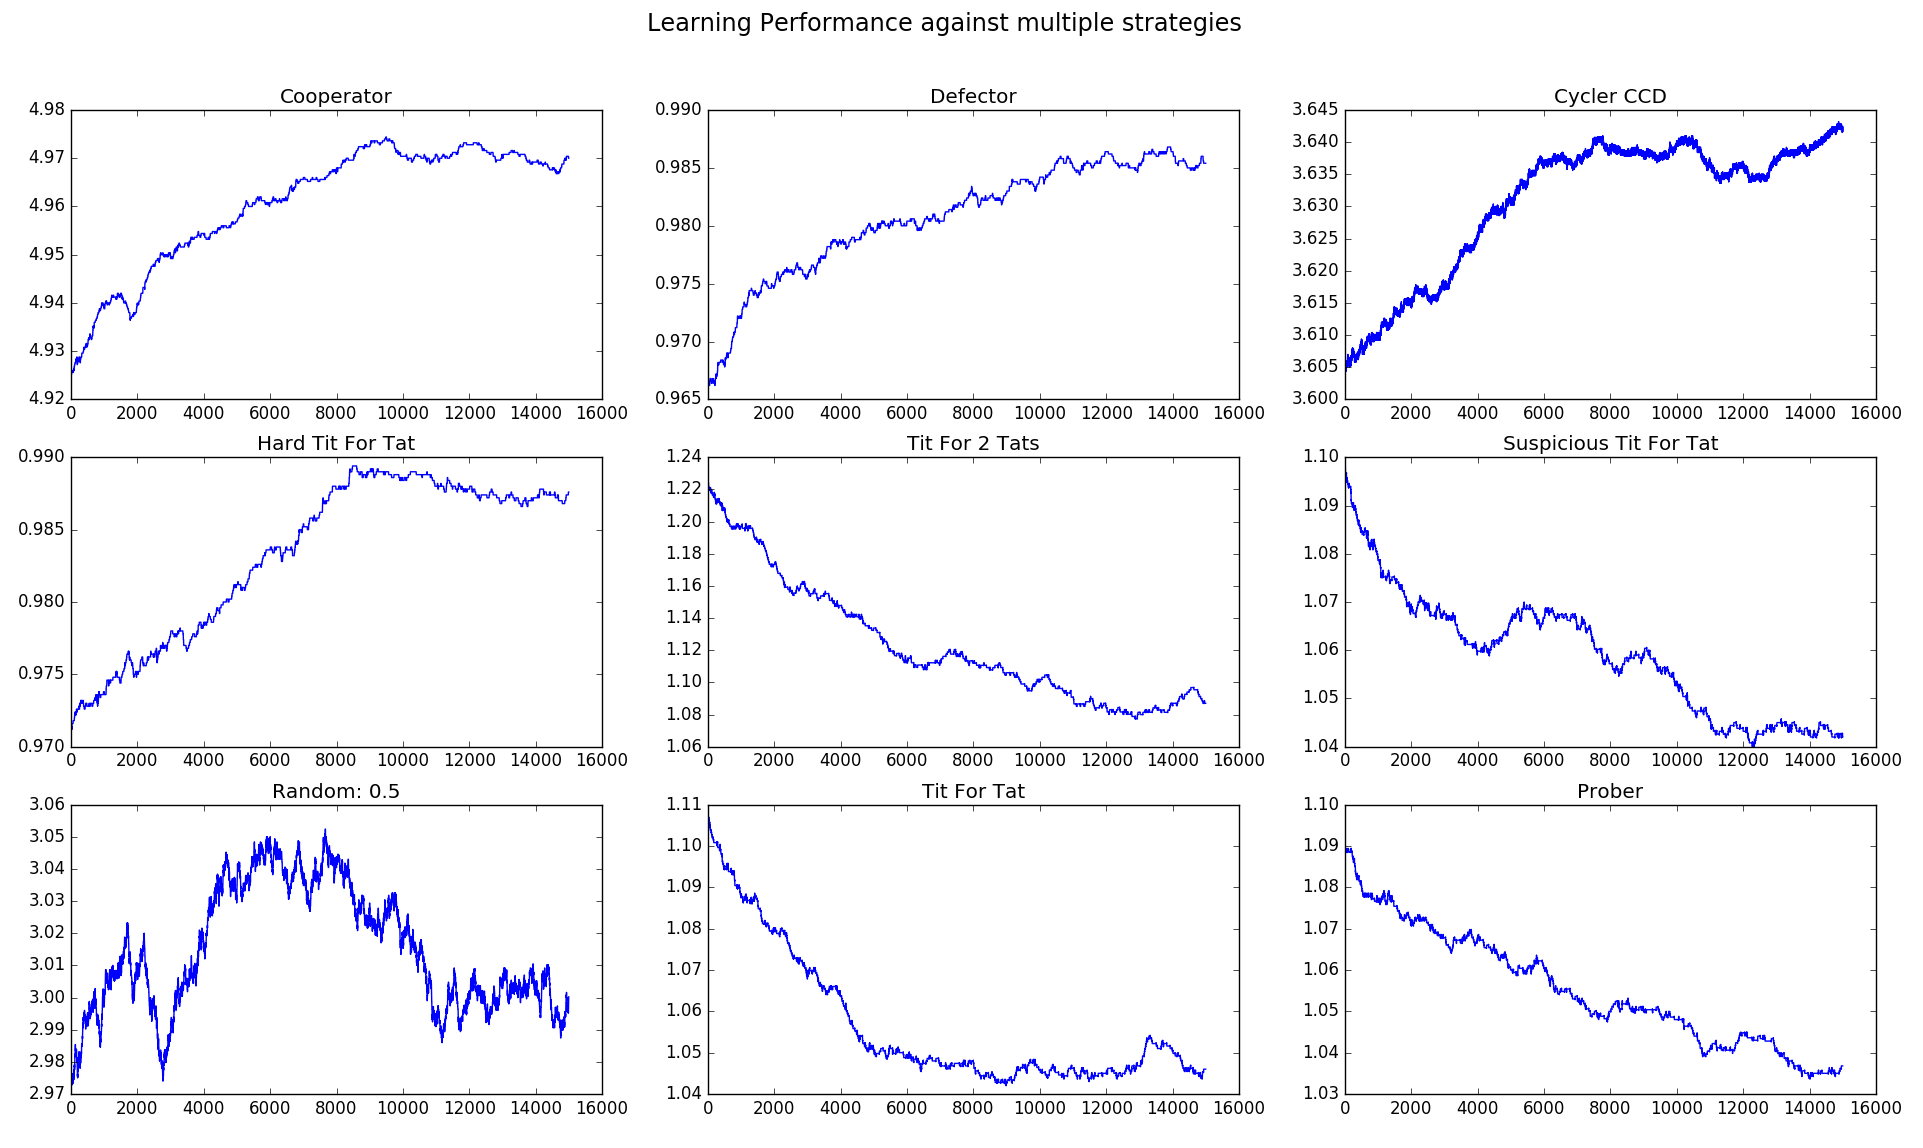
\includegraphics[width=\textwidth]{learnerInitialB.png}
	\caption{{Performance of Adaptive strategy (Variant B)}}
	\end{figure}

	As we can see, our strategy generally learns and improves its payoff. But in a few cases (Mostly against 'Tit for Tat' strategies), our strategy shows a slight (Notice the scale) decreasing trend. As we will discuss later, the reason for this is poor exploration. We try to exploit more instead of exploring, which leads to a very slight decrease in the payoff (Notice the scales in the plot).

	\begin{figure}[H]
	\centering
	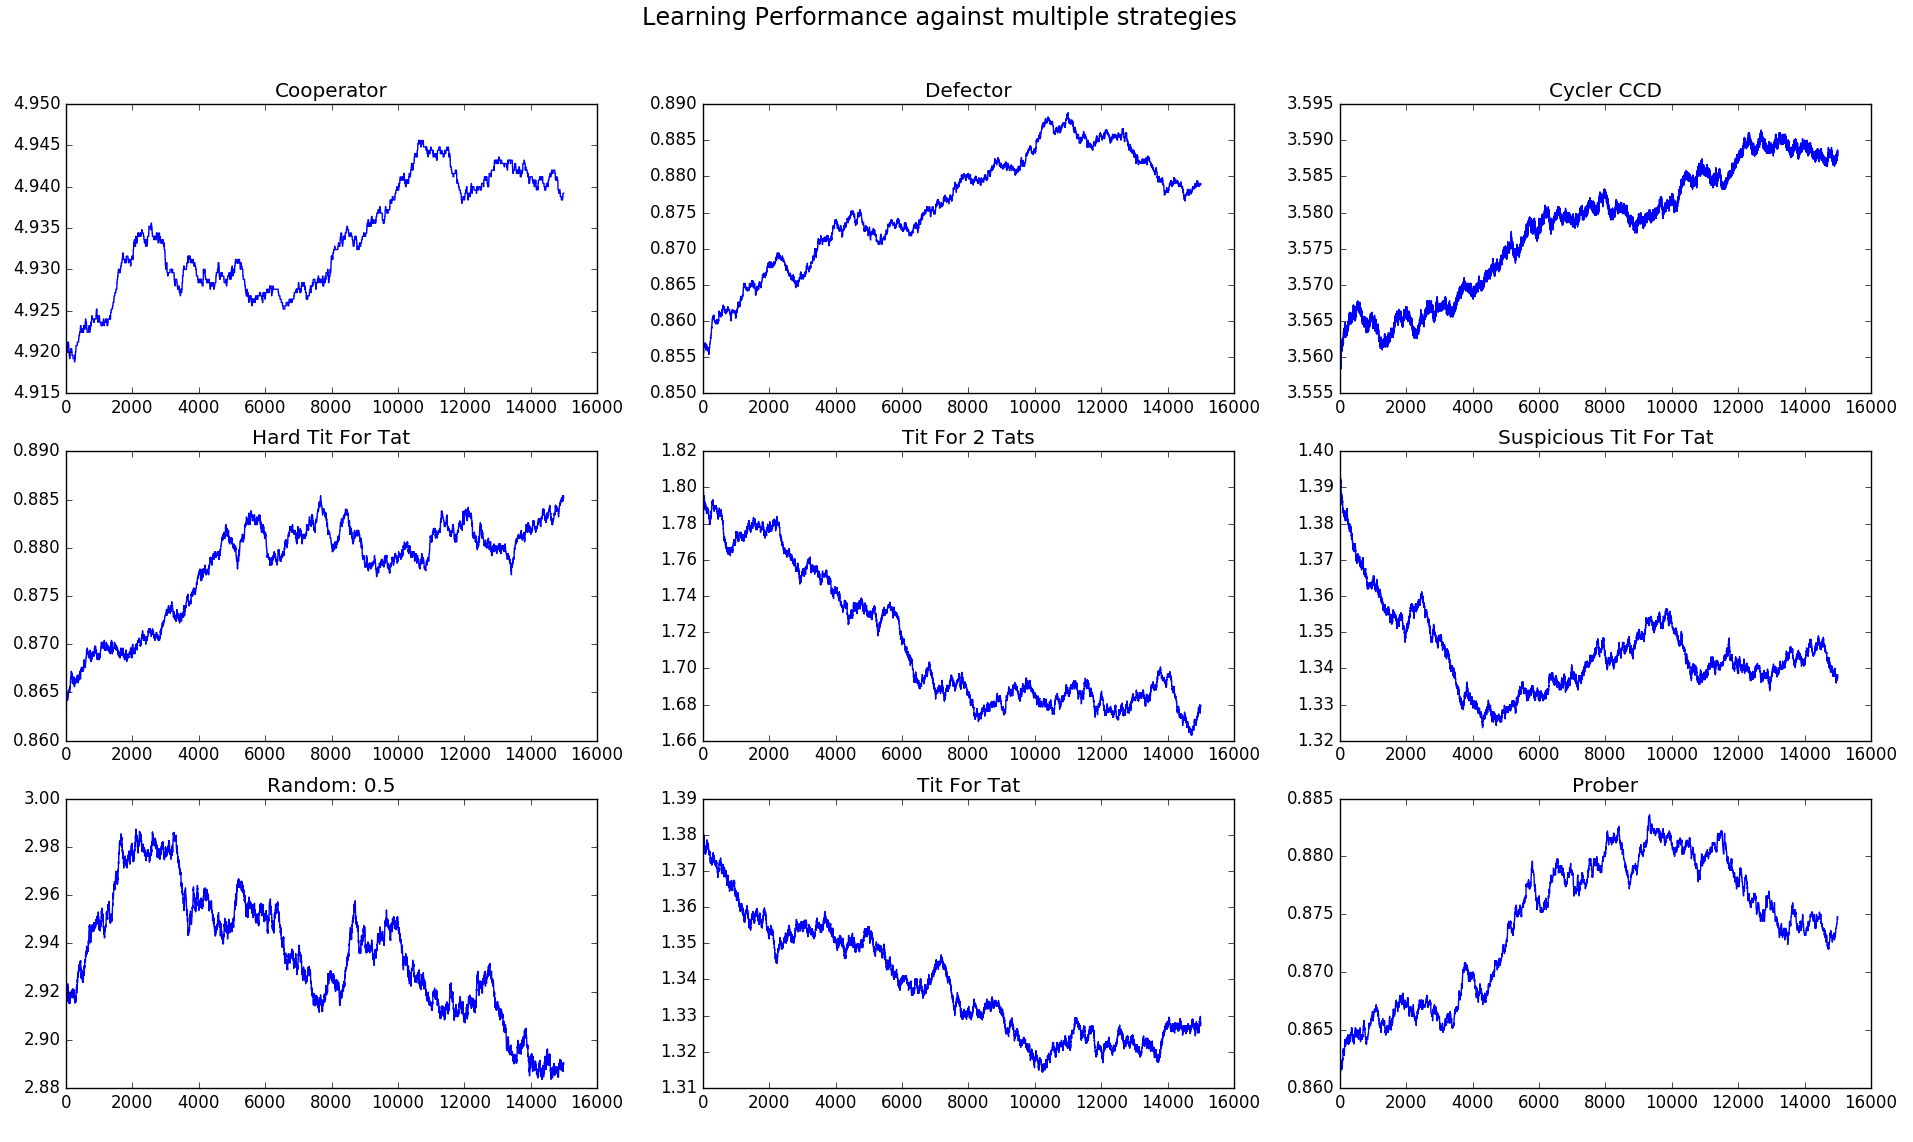
\includegraphics[width=\textwidth]{learnerInitialC_b8.png}
	\caption{{Performance of Adaptive strategy (Variant C)}}
	\end{figure}

	As we can see, Variant C is able to tackle the issue of decreasing payoffs to a certain extent. We'll have a more extensive discussion on this in future sections. Using softmax to incorporate exploration at each turn helps the model in continuing to learn. The 
	
	\subsection{Observations}
	
	\subsubsection{Effect of Parameters on Learning}

	As discussed earlier, using softmax drastically helps in improving the results. Here, we study the effect of the constant $c$ on the performance of the learning algorithm. Note that, a small $c$ neglects the role of the expected payoff while a higher $c$ makes its role even more important.

	\begin{figure}[H]
	\centering
	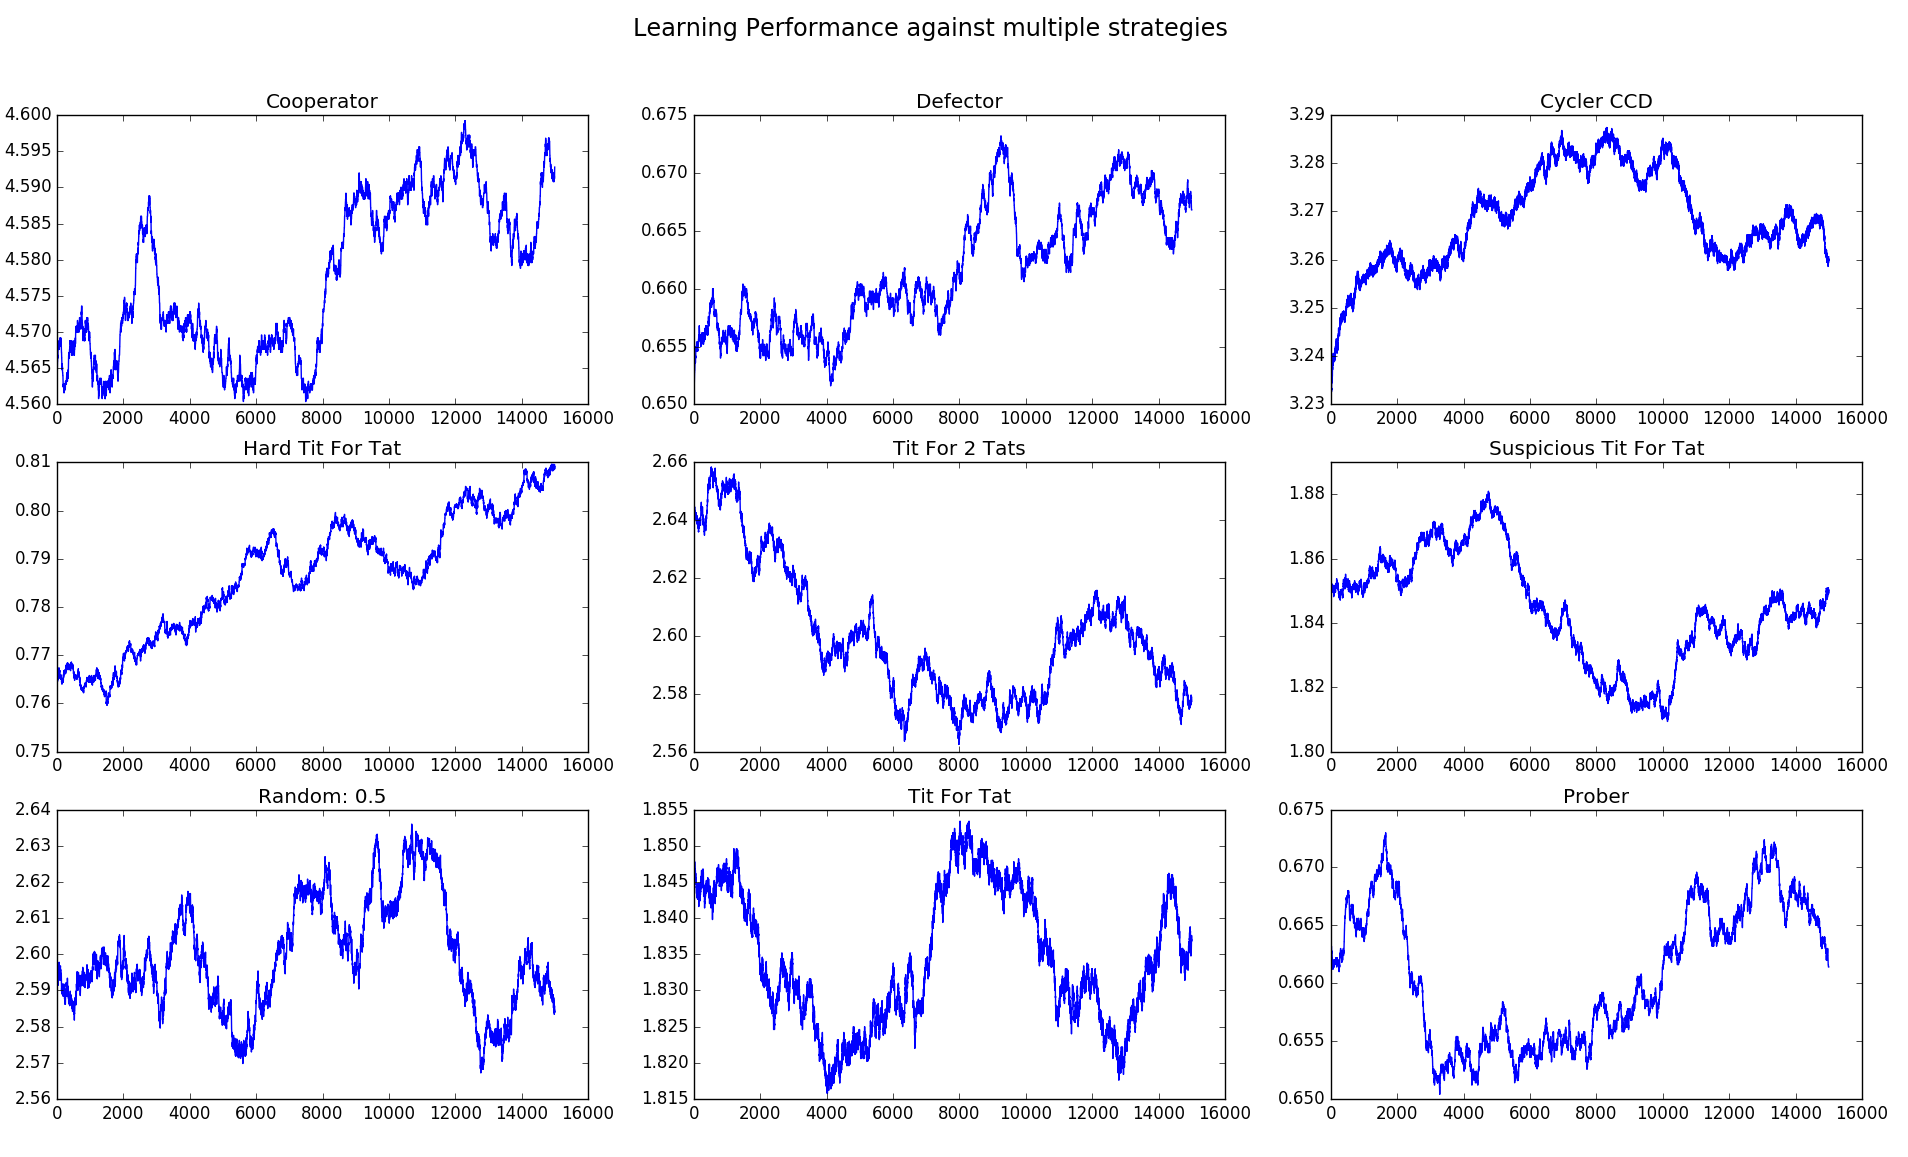
\includegraphics[width=\textwidth]{learnerInitialC_b2.png}
	\caption*{{Performance of Variant C ($c = 2$)}}
	\end{figure}
	
	As we can see, for $c=2$ there is almost no decreasing trend observed (Note that the fluctuations are extremely small). This is due to more emphasis on exploration instead of exploiting the current best move. Also note the higher payoffs observed in case of 'Tit for Tat' Strategies and also the slight drop in payoffs for the others.

	\begin{figure}[H]
	\centering
	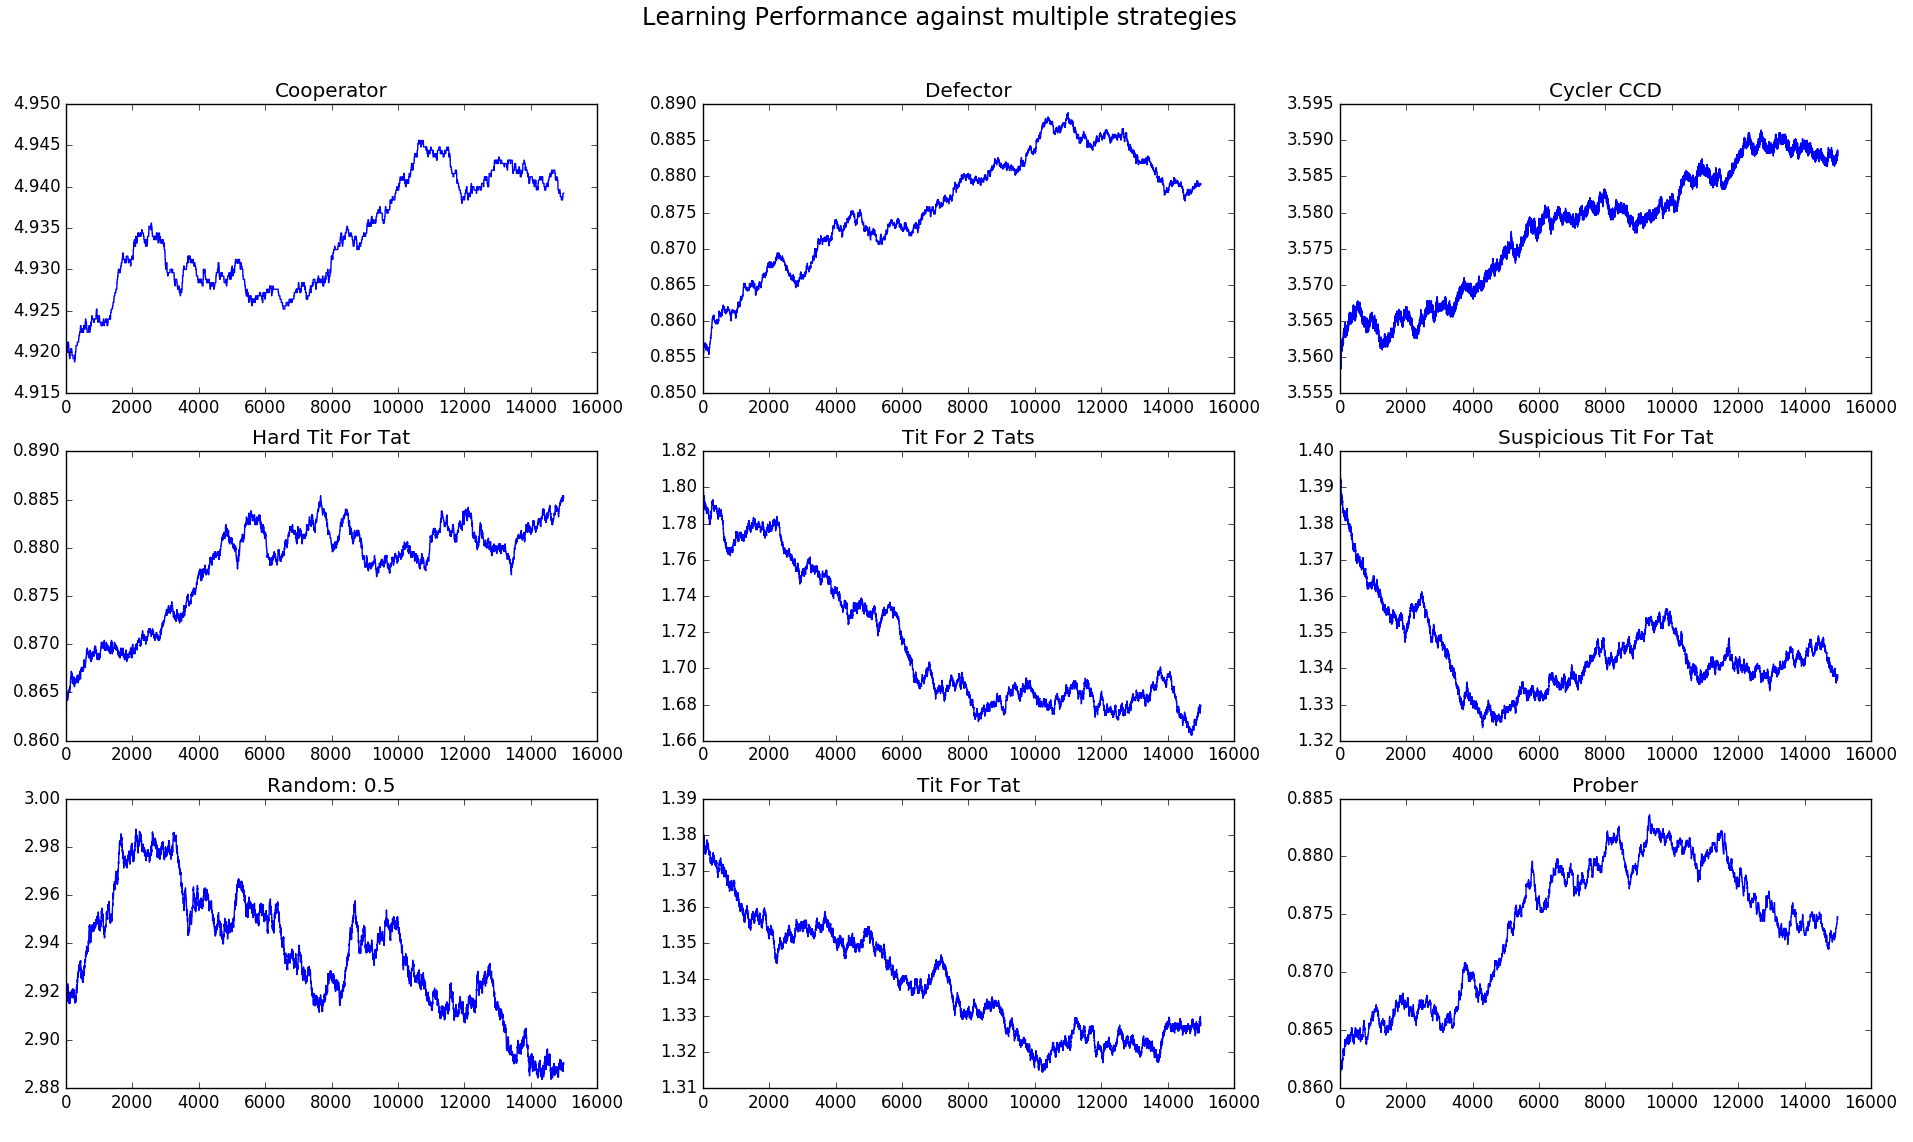
\includegraphics[width=\textwidth]{learnerInitialC_b8.png}
	\caption*{{Performance of Variant C ($c = 8$)}}
	\end{figure}

	\begin{figure}[H]
	\centering
	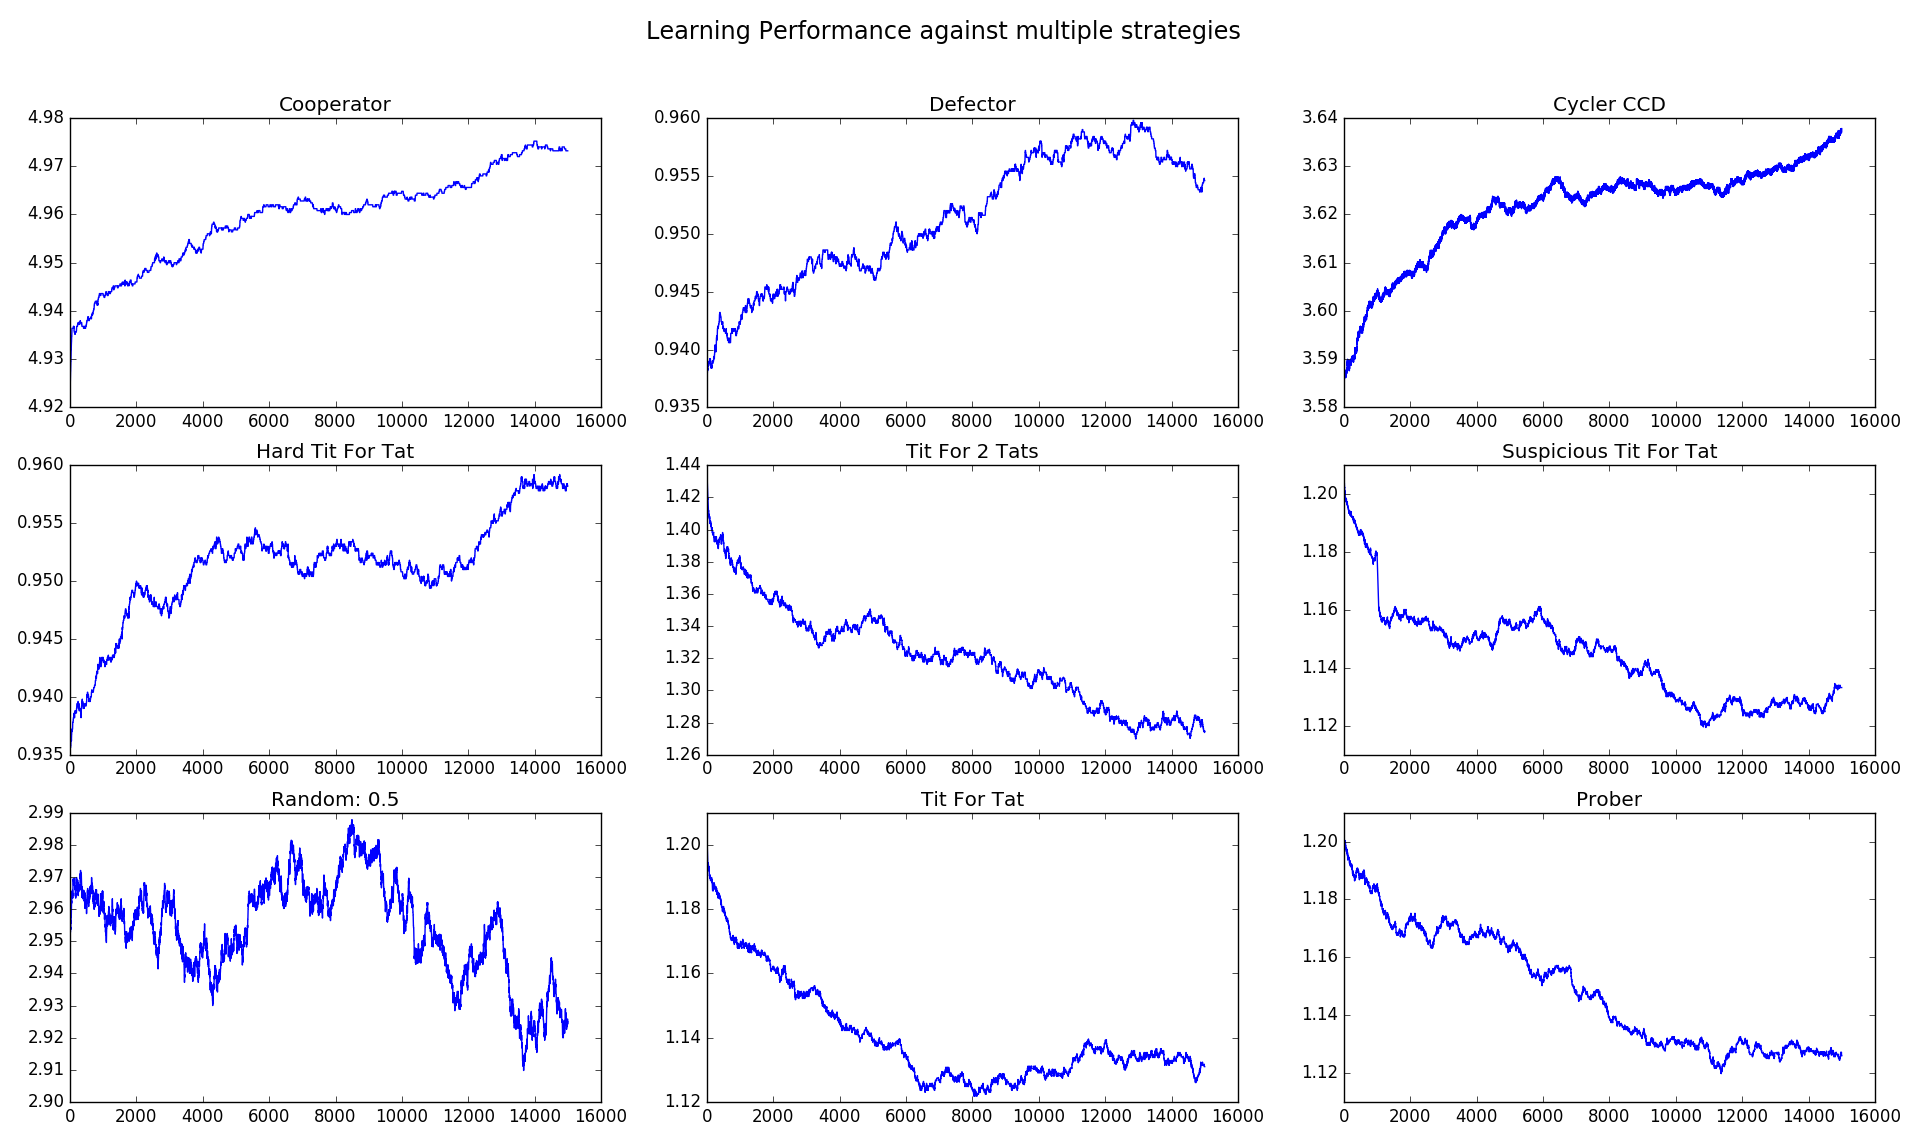
\includegraphics[width=\textwidth]{learnerInitialC_b32.png}
	\caption*{{Performance of Variant C ($c = 32$)}}
	\end{figure}

	With increasing $c$, the decreasing payoff effect becomes more prominent. Also, the payoffs for 'Tit for Tat' strategies decrease while it increases for the others.

	\subsubsection{Effect of Memory}
	
	Let's study the effect of memory on the performance of the adaptive strategy. It's evident that the number of states increase exponentially with memory length.	Consequently, the rate of learning will also be reduced accordingly since we have a larger number of unknowns which need to be estimated. The performance of the strategies for different memory lengths are shown below,\\
	
	\begin{table}[H]
	  \begin{center}
	    \begin{tabular}{|c|c|c|c|c|}
	      \toprule
		  \textsc{Memory Used} & \textsc{Cooperator} & \textsc{Defector} & {\footnotesize{\textsc{CyclerCCD}}} & \textsc{Hard TfT}\\
	      \midrule
		   1 & 	4.593 & 0.666 & 3.264 & 0.793\\
		   2 & 4.592 & 0.664 & \textbf{3.280} & 0.786\\
		   3 & 4.592 & 0.663 & \textbf{3.281} & 0.791\\
		   \bottomrule
	    \end{tabular}
	  \end{center}
	\end{table}  		

	\begin{table}[H]
	  \begin{center}
	    \begin{tabular}{|c|c|c|c|c|c|}
	      \toprule
	 	  \textsc{Memory Used} & \textsc{Tf2T} & {\footnotesize{\textsc{Suspicious TfT}}} & \textsc{Random} & \textsc{TfT} & \textsc{Prober}\\
	      \midrule
		  1	& 2.552 & 1.832 & 2.603 & 1.834 & 1.836\\
		  2 & \textbf{2.592} & 1.829 & 2.597 & 1.829 & 1.831\\
		  3 & \textbf{2.581} & 1.825 & 2.610 & 1.830 & 1.832\\
		\bottomrule
	    \end{tabular}
	  \end{center}
	\end{table}  		
	 
	As we can see from the above table, increasing memory has little or almost no effect on the performance of the strategy. This can be due to the fact that almost all the above strategies are extremely local in nature (i.e. Do not look more than 1-2 steps back). Thus, only one look up is enough to explain the opposing strategies well enough. This reasoning is supported by the fact that there is a slight improvement in the payoffs of the strategies  \textsc{CyclerCCD} and \textsc{Tit for 2 Tats}, both of which require at least 2-3 memory length to tackle efficiently.
	 
	\subsubsection{Special Cases: Cooperator and Defector}

	This section discusses the performance of our proposed adaptive strategy in detail by considering selective opponents i.e. Cooperator and Defector. We select these strategies for ease of discussion.\\
	
	\noindent
	\textbf{Cooperator: } As the name suggests, this is a simple strategy which always cooperates. Our algorithm starts off in a pure state, having no knowledge of what would be a better strategy. It interacts with the opponent and slowly learns which strategy give better returns. As can be seen in earlier figures, the strategy performs poorly initially (Due to no knowledge at the moment). Initially, it tries exploring all possible moves and infer which moves should be better. Thus, as observed in the plots, the payoffs slowly start to rise and approach 5 (The optimal value). In the end, the payoff is still slightly less than 5 due to a small amount of exploration being performed (To check whether another better strategy can be found).\\
	
	\noindent
	\textbf{Defector: } As the name suggests, this is a simple strategy which always defects. Note that against such a strategy, the maximum payoff is 1. 	Similar to the previous case, our algorithm starts off by having no previous knowledge. It interacts with the opponent and slowly learns which strategy give better returns. As can be seen in earlier figures, the strategy performs poorly initially (Due to exploration being performed). Thus, as observed in the plots and noted in the previous case, the payoffs slowly start to rise and approach 1 (The optimal value). Note that a defector will always win (In any case, against any strategy other then Defector itself) and consequently will always have higher (>=) payoff than the opponent. So, in effect our strategy has managed to learn the (nearly) best possible action in this case.

	\section{Showdown: Evolved Strategy Vs Adaptive Strategy}

	We perform matches between the Evolved strategies and the adaptive strategies to study their performance. We conduct matches of different length, to study both the initial and far-off behavior.
	
	\subsection{Performance Against Each Other}

	When the adaptive strategy is played against the evolved ones, the results are as follows,
	
	\begin{table}[H]
	  \begin{center}
	    \begin{tabular}{|c|c|c|}
	      \toprule
	 	  \textsc{Turns} & \textsc{Single Objective Strategy} & \textsc{Multi Objective Strategy}\\
	      \midrule
		  20    & \textbf{2.150} (1.400) & \textbf{2.400} (1.400)\\		  
		  200	& \textbf{2.190} (1.915) & \textbf{2.025} (1.725)\\
		  2000  & 1.827 \textbf{(2.017)} & 1.858 \textbf{(1.998)}\\
		  20000 & 1.781 \textbf{(1.95)} & 1.780 \textbf{(1.945)}\\
		  200000 & 1.743 \textbf{(1.962)} & 1.752 \textbf{(1.951)}\\
		\bottomrule
	    \end{tabular}
	  \end{center}
	\end{table}  		
	
	As we can see above, the adaptive strategy slowly adapts to the evolved strategy and starts outperforming them as the number of turns played increases. Note that the payoffs shown for turns = 20, 200 have extremely high variance and thus are not reliable (and should not be taken at face value).
	
	\subsection{Performance Against Other Strategies}
	
	\renewcommand{\tabcolsep}{8pt}

	\begin{table}[H]
	  \begin{center}
	    \begin{tabular}{|c|c|c|c|c|}
	      \toprule
	 	  \textsc{Strategy} & \textsc{Cooperator} & \textsc{Defector} & \textsc{CyclerCCD} & \textsc{Hard TfT}\\
		  \midrule
		  Adaptive Strategy & \textbf{4.932} \textbf{(0.102)} & 0.871 (1.514) & 3.577 (0.581) & 0.880 (1.524)\\
		  Single Obj & 4.000 (1.500) & \textbf{1.000 (1.000)} & \textbf{3.666 (0.334)} & \textbf{3.000 (3.000)}\\
		  Multi Obj & 4.000 (1.500) & \textbf{1.000 (1.000)} &  \textbf{3.666 (0.334)} & \textbf{3.000 (3.000)}\\
		\bottomrule
	    \end{tabular}
	  \end{center}
	\end{table}  		

	\renewcommand{\tabcolsep}{6pt}

	\begin{table}[H]
	  \begin{center}
	  	\footnotesize
	    \begin{tabular}{|c|c|c|c|c|c|}
	      \toprule
	 	  \textsc{Strategy} & \textsc{Tf2T} & {\footnotesize{\textsc{Suspicious TfT}}} & \textsc{Random} & \textsc{TfT} & \textsc{Prober}\\
		  \midrule
		  Adaptive Strategy & 1.710 {(1.205)} & 1.350 (1.350) & \textbf{2.904 (0.732)} & 1.360 (1.360) & 1.340 (1.340)\\
		  Single Obj & \textbf{4.000} \textbf{(1.500)} & \textbf{3.000 (3.000)} & 2.487 (1.710) & \textbf{3.000 (3.000)} & \textbf{3.000 (3.000)}\\
		  Mult Obj & \textbf{4.000} \textbf{(1.500)} & \textbf{3.000 (3.000)} & 2.488 (1.712) & \textbf{3.000 (3.000)} & \textbf{3.000 (3.000)}\\
		  \bottomrule
	    \end{tabular}
	  \end{center}
	\end{table}  		

	\section{Future Work}
			
	\section{References}

\end{document}


